%!TEX root = ../dissertation.tex
% this file is called up by thesis.tex
% content in this file will be fed into the main document

\graphicspath{{4-monophonic/figures/}}

\chapter{CREPE: Deep Monophonic Pitch Estimation}
\label{ch:monophonic}

As outlined in Chapter \ref{ch:introduction}, we start with a simpler formulation of music transcription that is later extended to ultimately support multi-instrument polyphonic music transcription.
This chapter concerns the first step where we assume that the input is monophonic, i.e. the audio contains at most one pitched sound at each instant.
Through this simplified formulation, we aim to gain insights on how a supervised learning framework for music transcription tasks can be designed.
Furthermore, we seek to identify important aspects of the proposed approach that can be applied to or extended to polyphonic and multi-instrument transcription tasks.
The content of this chapter is largely based on the work presented at IEEE ICASSP 2018 \cite{kim2018crepe}.

\section{Introduction}\label{sec:introduction}

Estimating the fundamental frequency (f0) of a monophonic audio signal, also known as pitch tracking or pitch estimation, is a long-standing topic of research in audio signal processing.
Pitch estimation plays an important role in music signal processing, where monophonic pitch tracking is used as a method to generate pitch annotations for multi-track datasets \cite{bittner2014medleydb} or as a core component of melody extraction systems \cite{bosch2014melody, mauch2015computer}. 
Pitch estimation is also important for speech analysis, where prosodic aspects such as intonations may reflect various features of speech \cite{zubizarreta1998prosody}.

\iffalse % (pasted in section II)
Computational methods for monophonic pitch estimation have been studied for more than a half-century \cite{noll1967cepstrum}, and many reliable methods have been proposed since.
Earlier methods commonly employ a certain candidate-generating function, accompanied by pre- and post-processing stages to produce the pitch curve.
Those functions include the cepstrum \cite{noll1967cepstrum}, the autocorrelation function (ACF) \cite{dubnowski1976acf}, the average magnitude difference function (AMDF) \cite{ross1974amdf}, the normalized cross-correlation function (NCCF) as proposed by RAPT \cite{talkin1995rapt} and PRAAT \cite{boersma1993praat}, and the cumulative mean normalized difference function as proposed by YIN \cite{decheveigne2002yin}. More recent approaches include SWIPE \cite{camacho2008swipe}, which performs template matching with the spectrum of a sawtooth waveform, and 
pYIN \cite{mauch2014pyin}, a probabilistic variant of YIN that uses a Hidden Markov Model (HMM) to decode the most probable sequence of pitch values.
According to a few comparative studies, the state of the art is achieved by YIN-based methods \cite{von2010comparison, babacan2013comparative}, with pYIN being the best performing method to date \cite{mauch2014pyin}.
\fi

We have reviewed a few approaches for monophonic pitch tracking in Section \ref{ch:mir}.\ref{sec:monophonic}, including YIN~\cite{decheveigne2002yin} and pYIN~\cite{mauch2014pyin}.
A notable trend in those methods is that the derivation of a better pitch detection system solely depends on cleverly devising a robust candidate-generating function and/or sophisticated post-processing steps, i.e.~heuristics, and none of them are directly learned from data, except for manual hyperparameter tuning.
This contrasts with many other problems in music information retrieval like chord ID \cite{humphrey2012rethinking} and beat detection \cite{bock2011enhanced}, where data-driven methods have been shown to consistently outperform heuristic approaches.
One possible explanation for this is that since fundamental frequency is a low-level physical attribute of an audio signal which is directly related to its periodicity, in many cases heuristics for estimating this periodicity perform extremely well with accuracies (measured in raw pitch accuracy, defined later on) close to 100\%, leading some to consider the task a solved problem.
This, however, is not always the case, and even top performing algorithms like pYIN can still produce noisy results for challenging audio recordings such as a sound of uncommon instruments or a pitch curve that fluctuates very fast.
This is particularly problematic for tasks that require a flawless f0 estimation, such as using the output of a pitch tracker to generate reference annotations for melody and multi-f0 estimation \cite{salamon2017analysis,bittner2017deepsalience}.

In the following sections, a novel, data-driven method for monophonic pitch tracking based on a deep convolutional neural network operating on the time-domain signal is presented.
This approach, CREPE (Convolutional  Representation  for  Pitch  Estimation), obtains state-of-the-art results, outperforming heuristic approaches such as pYIN and SWIPE while being more robust to noise too.
It is further shown that CREPE is highly precise, maintaining over 90\% raw pitch accuracy even for a strict evaluation threshold of just 10 cents.

\section{Architecture}

\begin{figure}
	\centering
	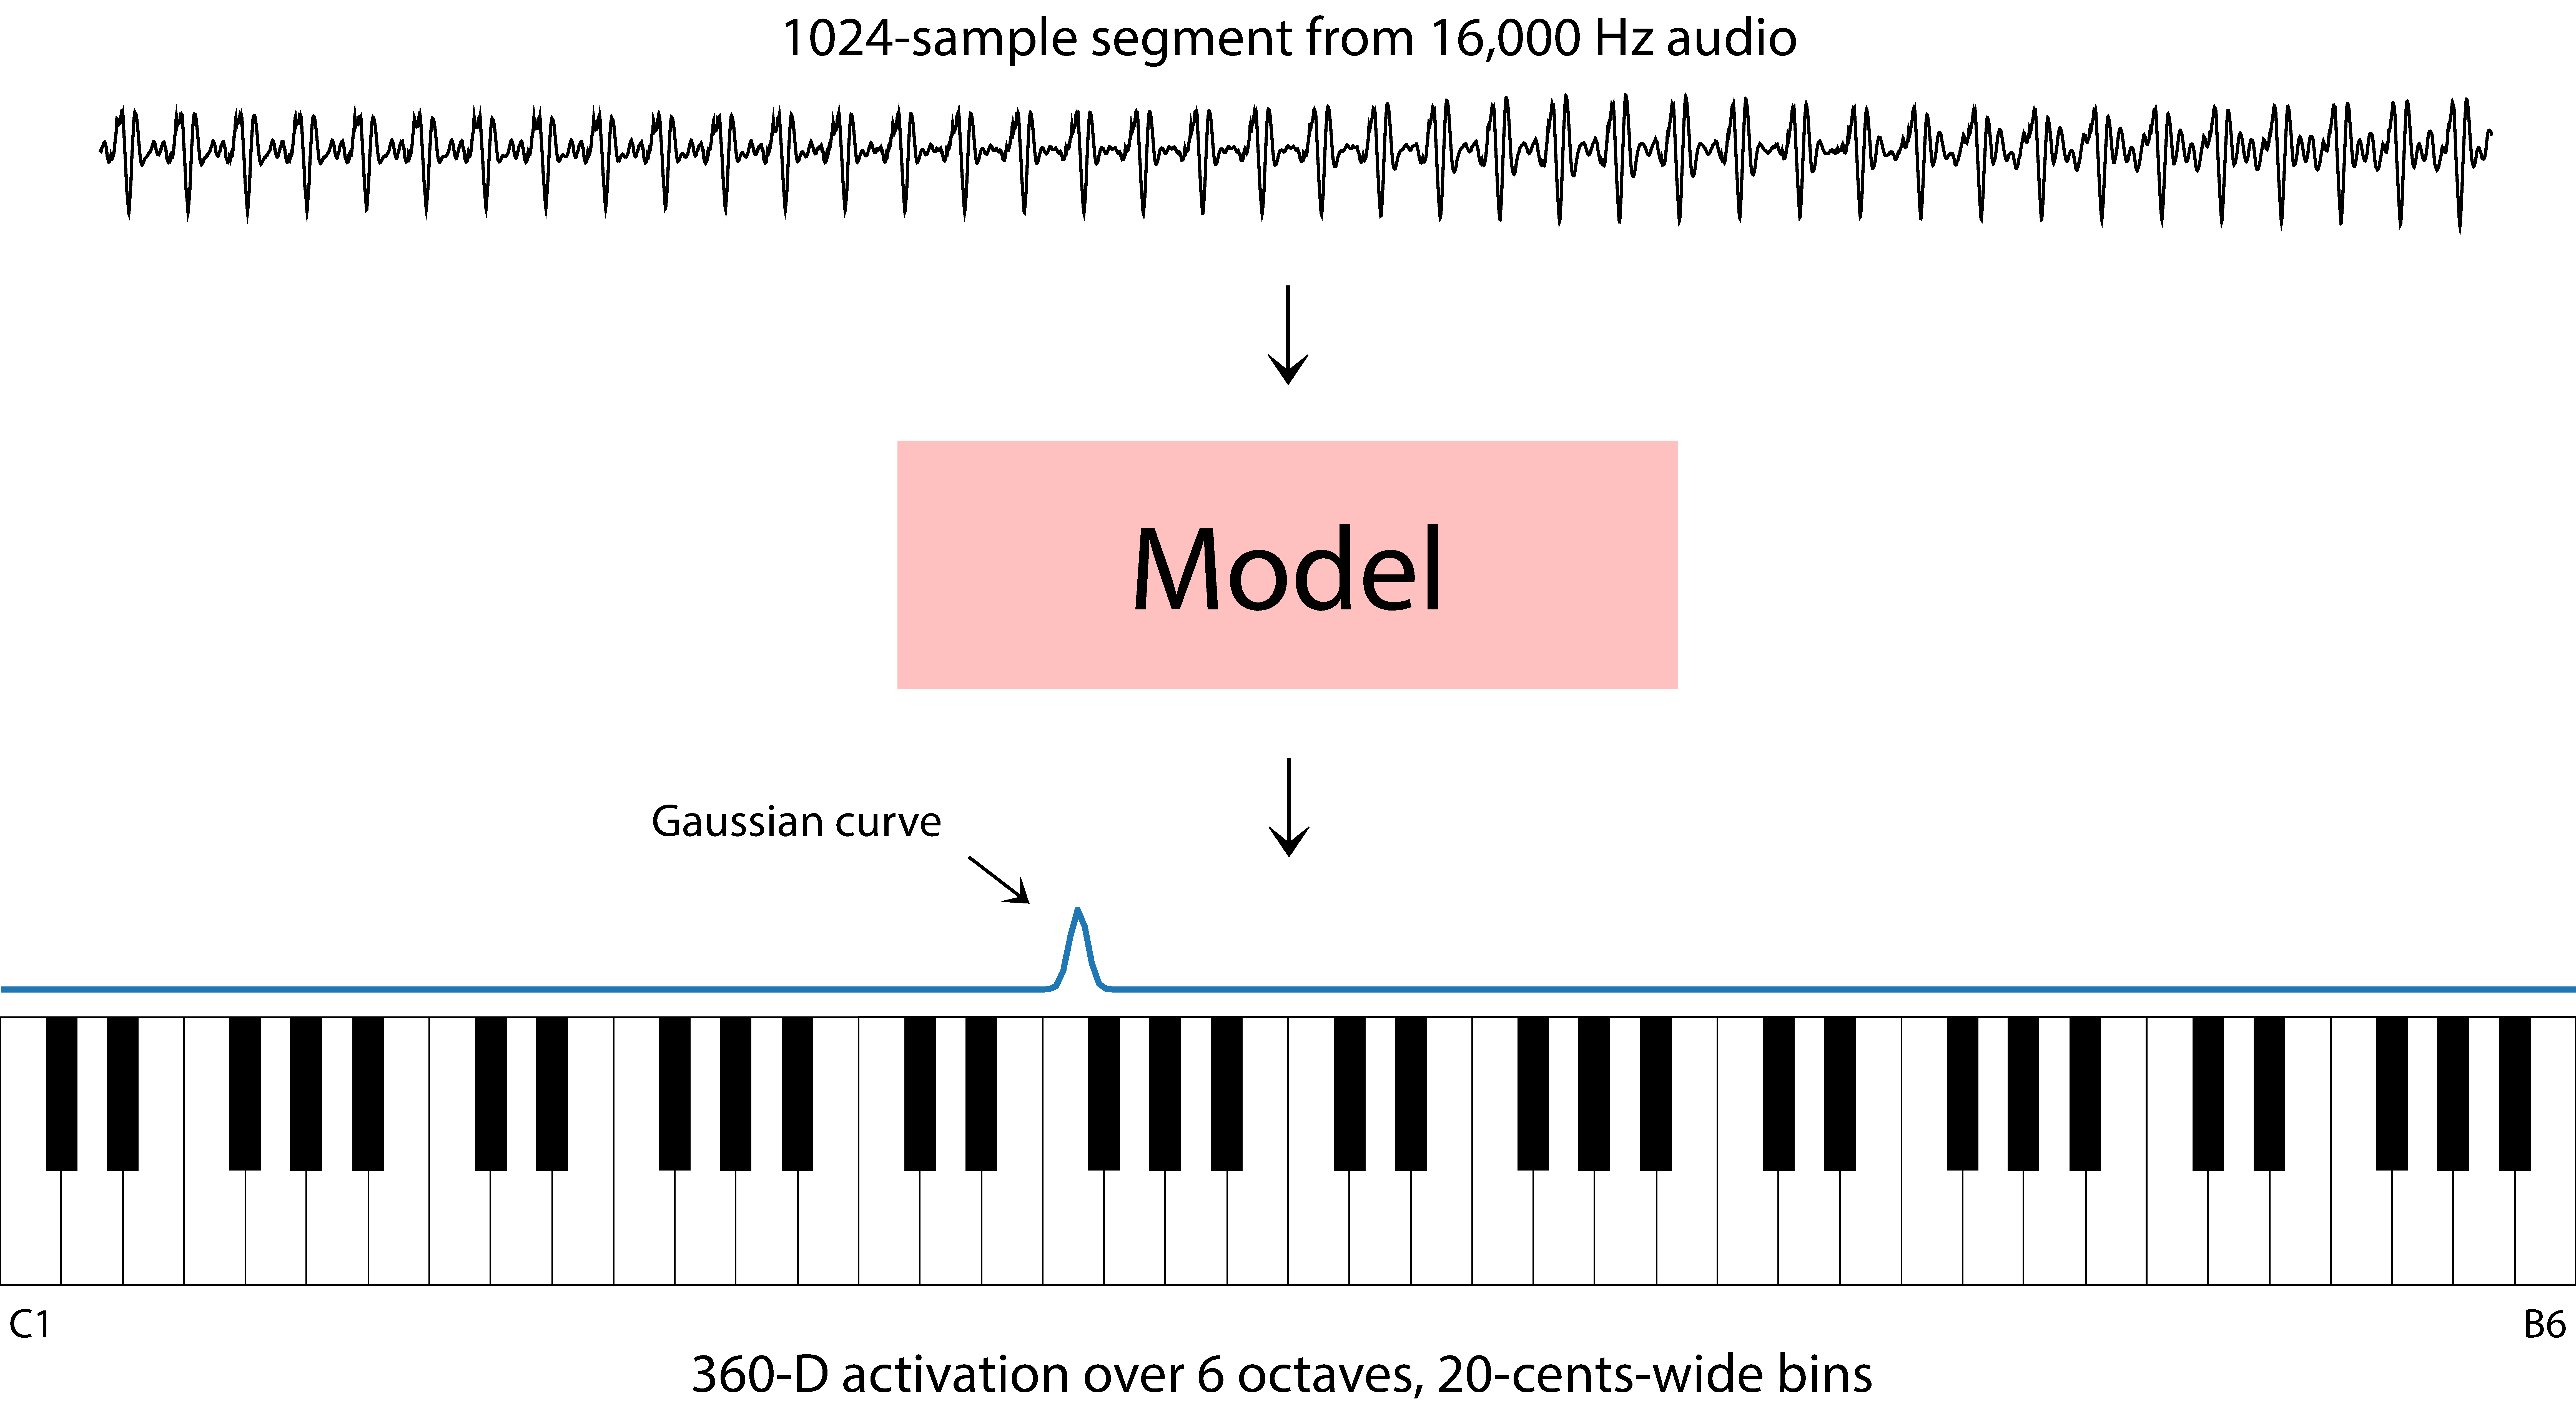
\includegraphics[width=0.9\linewidth]{formulation.pdf}
	\caption{The input and output representations of the CREPE model. The input is 1024 time-domain samples, and the output is a 360-dimensional vector that contains a Gaussian curve centered at the ground-truth frequency (see Equation \ref{eqn:gaussian}). For details on the convolutional architecture used in the model, see Figure \ref{fig:architecture}.}\label{fig:formulation}
\end{figure}

\begin{sidewaysfigure}
	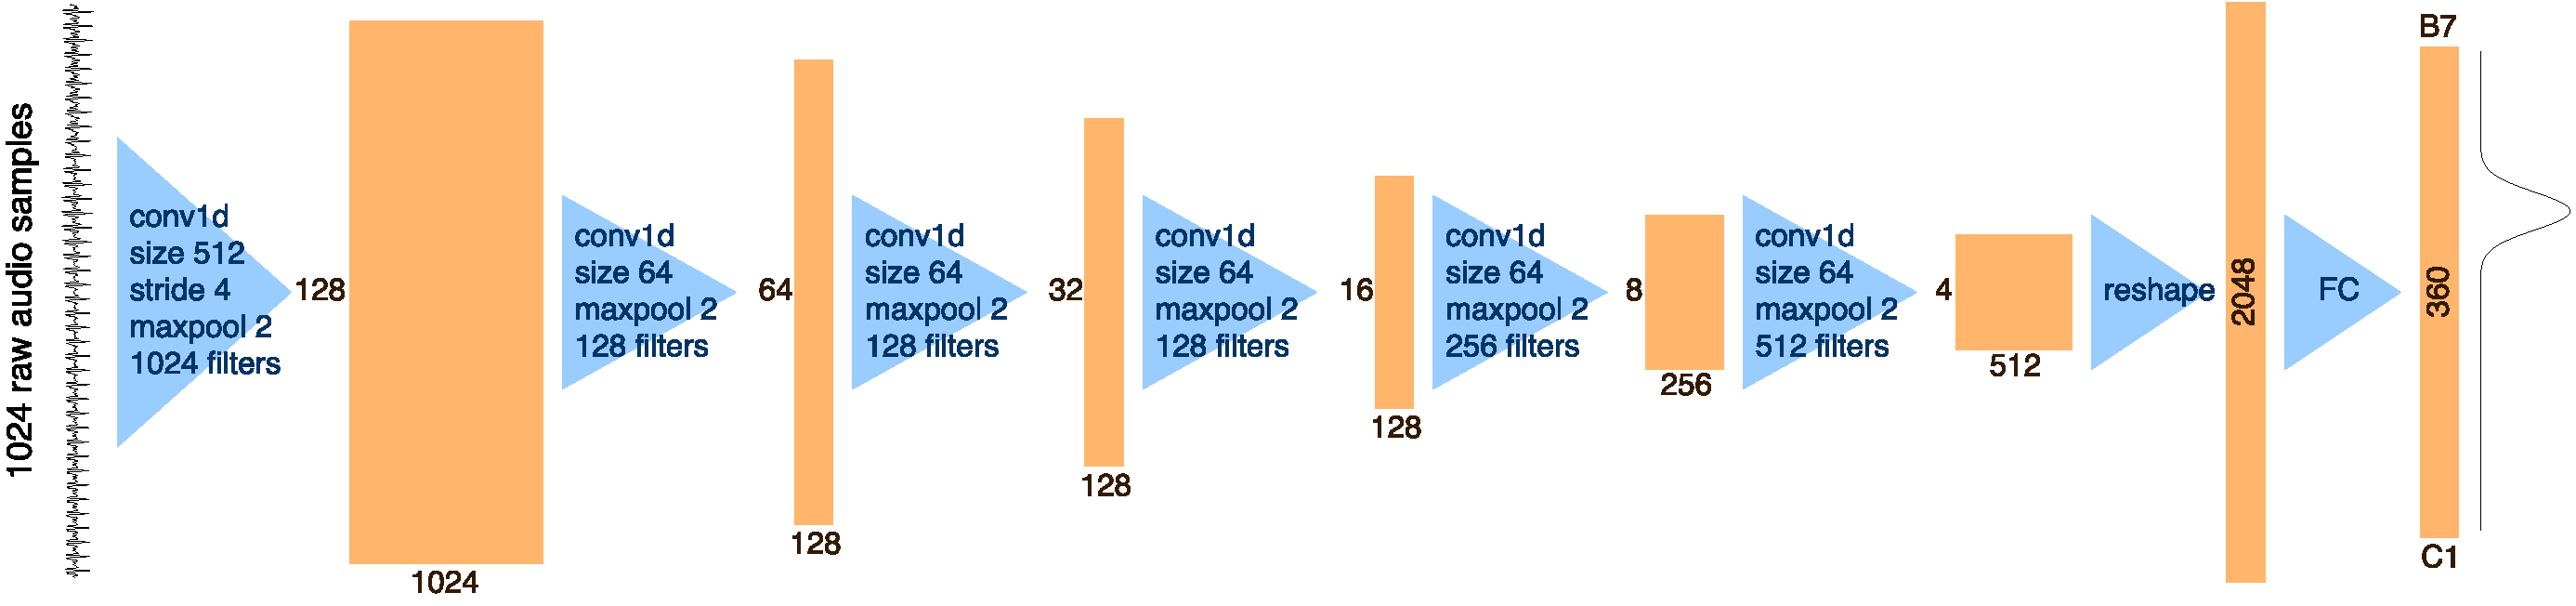
\includegraphics[width=\textwidth]{architecture.pdf}
	\caption{The architecture of the CREPE pitch tracker. The six convolutional layers predicts the Gaussian curve centered at the ground-truth frequency. The output is then used to extract the exact pitch estimate as in Equation \ref{eqn:resulting}-\ref{eqn:resulting2}.}
	\label{fig:architecture}
\end{sidewaysfigure}

CREPE consists of a deep convolutional neural network which operates directly on the time-domain audio signal to produce a pitch estimate.
The input and output representations used in the model are illustrated in Figure \ref{fig:formulation}.
The input is a 1024-sample excerpt from the time-domain audio signal, using a 16 kHz sampling rate, and the output is a 360-dimensional vector $\hat{\mathbf{y}}$, from which the resulting pitch estimate is calculated deterministically.

Each of the 360 dimensions in the output corresponds to a specific pitch value, defined in cents.
Cent is a unit representing musical intervals relative to a reference pitch $f_{\mathrm{ref}}$ in Hz, defined as a function of frequency $f$ in Hz:
\begin{equation}
\cent(f) = 1200 \cdot \log_2 \frac{f}{f_{\mathrm{ref}}},
\end{equation}
where $f_{\mathrm{ref}} = 10 \mathrm{~Hz}$ throughout the experiments. 
This unit provides a logarithmic pitch scale where 100 cents equal one semitone.
The 360 pitch values are denoted as $\cent_1, \cent_2, \cdots, \cent_{360}$ and are selected so that they cover six octaves with 20-cent intervals between C1 and B6, corresponding to 32.70 Hz and 1975.5 Hz. 
The resulting pitch estimate $\hat{\cent}$ is the weighted average of the associated pitches $\cent_i$ according to the output $\hat{\mathbf{y}}$, which gives the frequency estimate in Hz:
\begin{equation}\label{eqn:resulting}
\hat{\cent} = \frac{\sum_{i=1}^{360}\hat{y}_i \cent_i}{\sum_{i=1}^{360} \hat{y}_i},
\end{equation}
\begin{equation}\label{eqn:resulting2}
\hat{f} = f_{\mathrm{ref}} \cdot 2 ^ {\hat{\cent} / 1200}.
\end{equation}

The target outputs we use to train the model are 360-dimensional vectors, where each dimension represents a frequency bin covering 20 cents (the same as the model's output).
The bin corresponding to the ground truth fundamental frequency is given a magnitude of one.
As in \cite{bittner2017deepsalience}, in order to soften the penalty for near-correct predictions, the target is Gaussian-blurred in frequency such that the energy surrounding a ground truth frequency decays with a standard deviation of 25 cents:
\begin{equation}\label{eqn:gaussian}
y_i = \exp \left ( {-\frac{(\cent_i - \cent_{\mathrm{true}})^2}{2 \cdot 25^2}} \right ),
\end{equation}
This way, high activations in the last layer indicate that the input signal is likely to have a pitch that is close to the associated pitches of the nodes with high activations.

A detailed block diagram of the proposed architecture is provided in Figure \ref{fig:architecture}.
There are six convolutional layers that result in a 2048-dimensional latent representation, which is then connected densely to the output layer with sigmoid activations to produce the 360-dimensional target vector.
The network is trained to minimize the binary cross entropy between the target vector $\mathbf{y}$ and the predicted vector $\hat{\mathbf{y}}$:
\begin{equation}
\mathcal{L}(\mathbf{y}, \hat{\mathbf{y}}) = \sum_{i=1}^{360} \left ( - y_i \log \hat{y_i} - (1 - y_i) \log (1 - \hat{y_i}) \right ),
\end{equation}
where both $y_i$ and $\hat{y}_i$ are real numbers between 0 and 1.
This loss function is optimized using the ADAM optimizer \cite{kingma2015adam}, with the learning rate 0.0002. 
The best performing model is selected after training until the validation accuracy no longer improves for 32 epochs, where one epoch consists of 500 batches of 32 examples randomly selected from the training set. 
Each convolutional layer is preceded with batch normalization \cite{ioffe2015batchnorm} and followed by a dropout layer \cite{srivastava2014dropout} with the dropout probability 0.25.
This architecture and the training procedures are implemented using Keras \cite{chollet2015keras}.




\section{Experiments}

\subsection{Datasets}

In order to objectively evaluate CREPE and compare its performance to alternative algorithms, we require audio data with perfect ground truth annotations.
This is especially important since the performance of the compared algorithms is already very high.
In light of this, we cannot use a dataset such as MedleyDB \cite{bittner2014medleydb}, since its annotation process includes manual corrections which do not guarantee a 100\% perfect match between the annotation and the audio, and it can be affected, to a degree, by human subjectivity.
To guarantee a perfectly objective evaluation, we must use datasets of synthesized audio in which we have perfect control over the f0 of the resulting signal.
We use two such datasets: the first, RWC-synth, contains 6.16 hours of audio synthesized from the RWC Music Database \cite{goto2002rwc} and is used to evaluate pYIN in \cite{mauch2014pyin}.
It is important to note that the signals in this dataset were synthesized using a fixed sum of a small number of sinusoids, meaning that the dataset is highly homogenous in timbre and represents an over-simplified scenario.
To evaluate the algorithms under more realistic (but still controlled) conditions, the second dataset we use is a collection of 230 monophonic stems taken from MedleyDB and re-synthesized using the methodology presented in \cite{salamon2017analysis}, which uses an analysis/synthesis approach to generate a synthesized track with a perfect f0 annotation that maintains the timbre and dynamics of the original track.
This dataset consists of 230 tracks with 25 instruments, totaling 15.56 hours of audio, and henceforth referred to as MDB-stem-synth.


\subsection{Methodology}

We train the model using 5-fold cross-validation, using a 60/20/20 train, validation, and test split.
For MDB-stem-synth, we use artist-conditional folds, in order to avoid training and testing on the same artist which can result in artificially high performance due to artist or album effects \cite{sturm2013classification}.
The evaluation of an algorithm's pitch estimation is measured in raw pitch accuracy (RPA) and raw chroma accuracy (RCA) with 50 cent thresholds \cite{salamon2014melody}.
These metrics measure the proportion of frames in the output for which the output of the algorithm is within 50 cents (a quarter-tone) of the ground truth.
We use the reference implementation provided in \texttt{mir\_eval} \cite{raffel2014mir_eval} to compute the evaluation metrics.

We compare CREPE against the current state of the art in monophonic pitch tracking, represented by the pYIN \cite{mauch2014pyin} and SWIPE \cite{camacho2008swipe} algorithms.
To examine the noise robustness of each algorithm, we also evaluate their pitch tracking performance on degraded versions of MDB-stem-synth, using the Audio Degradation Toolbox (ADT) \cite{mauch2013adt}.
We use four different noise sources provided by the ADT: pub, white, pink, and brown.
The pub noise is an actual recording of the sound in a crowded pub, 
and the white noise is a random signal with a constant power spectral density over all frequencies.
The pink and brown noise have the highest power spectral density in low frequencies, and the densities fall off at 10 dB and 20 dB per decade respectively.
Seven different signal-to-noise ratio (SNR) values are used: $\infty$, 40, 30, 20, 10, 5, and 0 dB.


\subsection{Results}

\subsubsection{Pitch Accuracy}

Table \ref{tbl:accuracy50} shows the pitch estimation performance tested on the two datasets.
On the RWC-synth dataset, CREPE yields a close-to-perfect performance where the error rate is lower than the baselines by more than an order of magnitude.
While these high accuracy numbers are encouraging, those are achievable thanks to the highly homogeneous timbre of the dataset.
In order to test the generalizability of the algorithms on a more timbrally diverse dataset, the performance is evaluated on the MDB-stem-synth dataset as well.
It is notable that the degradation of performance from RWC-synth is more significant for the baseline algorithms, implying that CREPE is more robust to complex timbres compared to pYIN and SWIPE.

\begin{table}[t]
	\begin{center}
		\begin{tabular}{c|c||c|c|c} \hline
			\multicolumn{1}{c}{Dataset} & \multicolumn{1}{c}{Metric} & \multicolumn{1}{c}{CREPE} & \multicolumn{1}{c}{pYIN} & \multicolumn{1}{c}{SWIPE} \\ \hline
			\multirow{2}{*}{RWC-synth} & RPA & \textbf{0.999$\pm$0.002} & 0.990$\pm$0.006& 0.963$\pm$0.023 \\ \cline{2-5}
			& RCA & \textbf{0.999$\pm$0.002} & 0.990$\pm$0.006& 0.966$\pm$0.020 \\ \hline \hline
			\multirow{2}{*}{MDB-stem-synth} & RPA & \textbf{0.967$\pm$0.091} & 0.919$\pm$0.129& 0.925$\pm$0.116 \\ \cline{2-5}
			& RCA & \textbf{0.970$\pm$0.084} & 0.936$\pm$0.092& 0.936$\pm$0.100 \\ \hline
		\end{tabular}
	\end{center}
	\caption{Average raw pitch/chroma accuracies and their standard deviations, tested with the 50 cents threshold.}
	\label{tbl:accuracy50}
\end{table}

\begin{table}[t]
	\begin{center}
		\begin{tabular}{c|c||c|c|c} \hline
			\multicolumn{1}{c}{Dataset} & \multicolumn{1}{c}{Threshold} &  \multicolumn{1}{c}{CREPE} & \multicolumn{1}{c}{pYIN} & \multicolumn{1}{c}{SWIPE} \\ \hline
			
			\multirow{3}{*}{RWC-synth} 
			& 50 cents & \textbf{0.999$\pm$0.002} & 0.990$\pm$0.006 & 0.963$\pm$0.023 \\ \cline{2-5}
			& 25 cents & \textbf{0.999$\pm$0.003} & 0.972$\pm$0.012 & 0.949$\pm$0.026 \\ \cline{2-5}
			& 10 cents & \textbf{0.995$\pm$0.004} & 0.908$\pm$0.032 & 0.833$\pm$0.055 \\ \hline \hline
			
			\multirow{3}{*}{MDB-stem-synth}
			& 50 cents & \textbf{0.967$\pm$0.091} & 0.919$\pm$0.129 & 0.925$\pm$0.116 \\ \cline{2-5}
			& 25 cents & \textbf{0.953$\pm$0.103} & 0.890$\pm$0.134 & 0.897$\pm$0.127 \\ \cline{2-5}
			& 10 cents & \textbf{0.909$\pm$0.126} & 0.826$\pm$0.150 & 0.816$\pm$0.165 \\ \hline
		\end{tabular}
	\end{center}
	\caption{Average raw pitch accuracies and their standard deviations, with different evaluation thresholds.}
	\label{tbl:thresholds}
\end{table}

Finally, to see how the algorithms compare under scenarios where any deviation in the estimated pitch from the true value could be detrimental, Table \ref{tbl:thresholds} reports the RPA at lower evaluation tolerance thresholds of 10 and 25 cents as well as the RPA at the standard 50 cents threshold for reference.
The table indicates that as the threshold is decreased, the difference in performance becomes more accentuated, with CREPE outperforming by over 8 percentage points when the evaluation tolerance is lowered to 10 cents.
The high accuracy in 10 cents despite the 20-cent resolution of the model output indicates that the weighted average solution in Equation \ref{eqn:resulting} is effective at predicting the precise frequencies even between the adjacent frequency bins.
This suggests that CREPE is especially preferable when even minor deviations from the true pitch should be avoided as best as possible.
Obtaining highly precise pitch annotations is perceptually meaningful for transcription and analysis/resynthesis applications.


\subsubsection{Noise Robustness}


Noise robustness is key to many applications like speech analysis for mobile phones or smart speakers, or for live music performance.
Figure \ref{fig:noise} shows how the pitch estimation performance is affected when an additive noise is present in the input signal.
CREPE maintains the highest accuracy for all SNR levels for pub noise and white noise, and for all SNR levels except for the highest level of pink noise.
Brown noise is the exception where pYIN's performance is almost unaffected by the noise.
This can be attributed to the fact that brown noise has most of its energy at low frequencies, to which the YIN algorithm (on which pYIN is based) is particularly robust.

\begin{sidewaysfigure}
	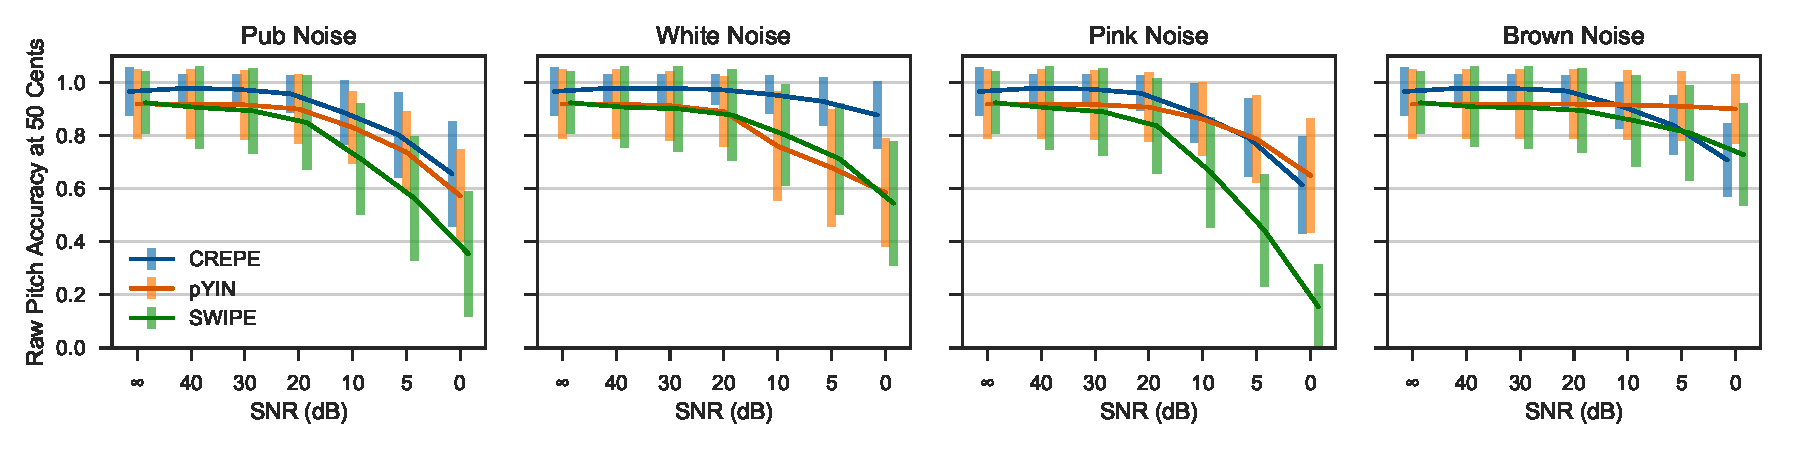
\includegraphics[width=\textwidth]{noise.pdf}
	\caption{Pitch tracking performance when additive noise signals are present. The error bars are centered at the average raw pitch accuracies and span the first standard deviations. With brown noise being a notable exception, CREPE shows the highest noise robustness in general. }
	\label{fig:noise}
\end{sidewaysfigure}

To summarize, CREPE performs better in all cases where the SNR is below 10 dB while the performance varies depending on the spectral properties of the noise when the noise level is higher, which indicates that this approach can be reliable under a reasonable amount of additive noise.
CREPE is also more stable, exhibiting consistently lower variance in performance compared to the baseline algorithms.


\begin{figure}
	\begin{minipage}{\columnwidth}
		\begin{center}
			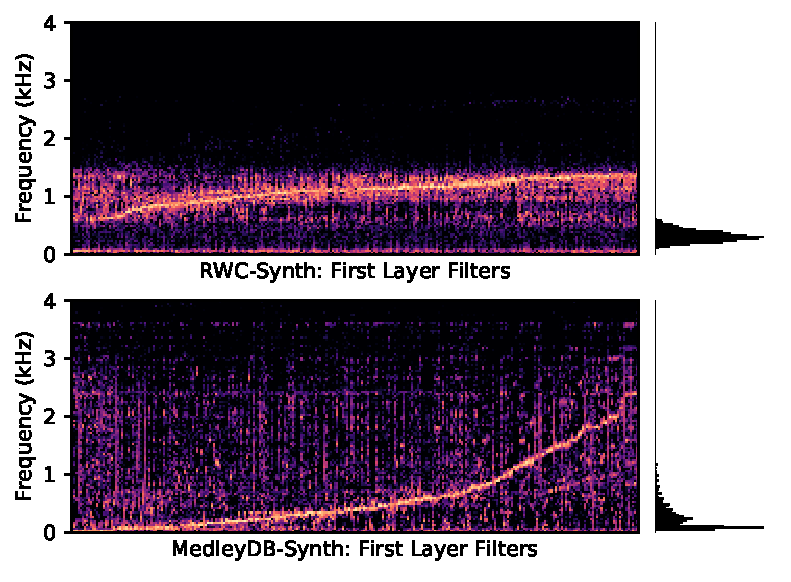
\includegraphics[width=0.8\columnwidth]{firstlayer-45.pdf}
		\end{center}
		\vspace{-10pt}
		\caption{
			Fourier spectra of the first-layer filters sorted by the frequency of the peak magnitude.
			Histograms on the right show the distribution of ground-truth frequencies in the corresponding dataset.
		}
		\label{fig:firstlayer}
	\end{minipage}
	\\ \vspace{2em} \\ 
	\begin{minipage}{\columnwidth}
		\begin{center}
			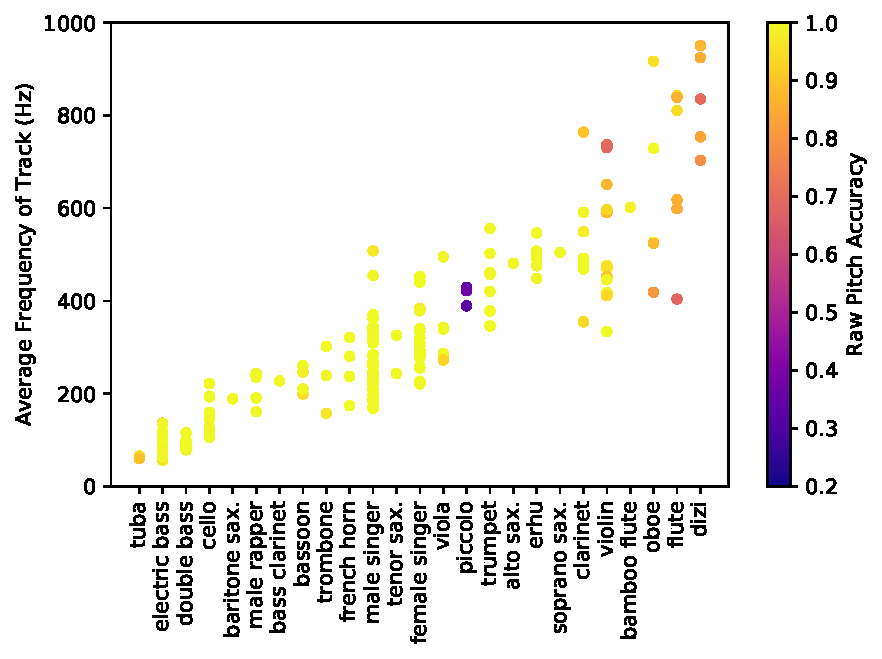
\includegraphics[width=0.8\columnwidth]{per-track-inst-45.pdf}
		\end{center}
		\vspace{-10pt}
		\caption{
			The raw pitch accuracy (RPA) of CREPE's predictions on each of the 230 tracks in MDB-stem-synth with respect to the instrument, sorted by the average frequency.
			% The  low-performing  cases  are  concentrated  in  the extreme frequencies, showing that the model performs better for the sfrequency range that are well-represented in the training set.
		}
		\label{fig:per-track}
	\end{minipage}
\end{figure}


\subsubsection{Model Analysis}

To gain some insight into the CREPE model, we visualize in Figure \ref{fig:firstlayer} the spectra of the 1024 convolutional filters in the first layer of the neural network, with histograms of the ground-truth frequencies to the right of each plot.
It is noticeable that the filters learned from the RWC-synth dataset have the spectral density concentrated between 600 Hz and 1500 Hz, while the ground-truth frequencies are mostly between 100 Hz and 600 Hz.
This indicates that the first convolutional layer in the model learns to distinguish the frequencies of the overtones rather than the fundamental frequency.
These filters focusing on overtones are also visible for MDB-stem-synth, where peak frequencies of the filters range well above the f0 distribution of the dataset, but in this case, the majority of the filters overlap with the ground-truth distribution, unlike RWC-synth.
A possible explanation for this is that since the timbre in RWC-synth is fixed and identical for all tracks, the model is able to obtain a highly accurate estimate of the f0 by modeling its harmonics.
Conversely, when the timbre is heterogeneous and more complex, as is the case for MDB-stem-synth, the model cannot rely solely on the harmonic structure and requires filters that capture the f0 periodicity directly in addition to the harmonics.
In both cases, this suggests that the neural network can adapt to the distribution of timbre and frequency in the dataset of interest, which in turn contributes to the higher performance of CREPE compared to the baseline algorithms.

\subsubsection{Performance by Instrument}

The MDB-stem-synth dataset contains 230 tracks from 25 different instruments, where electric bass (58 tracks) and male singer (41 tracks) are the most common while there are instruments that occur in only one or two tracks.
Figure \ref{fig:per-track} shows the performance of CREPE on each of the 230 tracks, with respect to the instrument of each track.
It is notable that the model performs worse for the instruments with higher average frequencies, but the performance is also dependent on the timbre.
CREPE performs particularly worse on the tracks with the dizi, a Chinese transverse flute, because the tracks came from the same artist, and they are all placed in the same split.
This means that for the fold in which the dizi tracks are in the test set, the training and validation sets do not contain a single dizi track, and the model fails to generalize to this previously unseen timbre.
There are 5 instruments (bass clarinet, bamboo flute, and the family of saxophones) that occur only once in the dataset, but their performance is decent, because their timbres do not deviate too far from other instruments in the dataset.
For the flute and the violin, although there are many tracks with the same instrument in the training set, the performance is low when the sound in the tested tracks is too low (flute) or too high (violin) compared to other tracks of the same instruments.
The low performance on the piccolo tracks is due to an error in the dataset where the annotation is inconsistent with the correct pitch range of the instrument.
Unsurprisingly, the model performs well on test tracks whose timbre and frequency range are well-represented in the training set.

\section{Open-Sourcing CREPE}

Releasing an implementation of research work as an open-source software helps ensure better quality, reproducibility, and longevity of the research code~\cite{mcfee2019opensource}.
To facilitate easier adoption of CREPE's pitch tracking functionality for wider audience, we open-sourced\footnote{\url{https://github.com/marl/crepe}} the implementation of CREPE under the MIT License.
The main purpose of the open-source release is to make the usage of the CREPE software as easy and effective as possible, so we aimed to ensure that the pitch estimation can work accurately for the broad range of the real-world monophonic signals.
As shown in Figure \ref{fig:firstlayer}, a model trained on a specific dataset specializes to the characteristics of the sounds in the dataset and will fail to work well across the previously unknown, real-world inputs.
To address this problem, we used six different datasets for the pre-trained model included in the open-source release of CREPE: MIR-1K~\cite{hsu2010mir1k}, Bach10~\cite{duan2010bach10}, RWC-Synth~\cite{mauch2014pyin}, MedleyDB~\cite{bittner2014medleydb}, MDB-STEM-Synth~\cite{salamon2017analysis}, and NSynth~\cite{engel2017nsynth}.
These datasets contain various instrumental and vocal sounds, and the pre-trained model is expected to work well on these types of sounds.
A visualization of the first-layer filters for the model trained with these datasets are shown in Figure \ref{fig:firstlayer-one}.
Compared to Figure \ref{fig:firstlayer}, the peak-frequency curve better covers the full range of frequencies and in a smoother manner.
An interesting feature of this visualization is that the curve is somewhat linear until 1 kHz and rapidly grows for the higher frequencies.
This roughly coincides with the Mel scale, where the mapping from the perceived frequency to the actual frequency is linear below 1 kHz and logarithmic above~\cite{logan2000mfcc}.


\begin{figure}
	\centering
	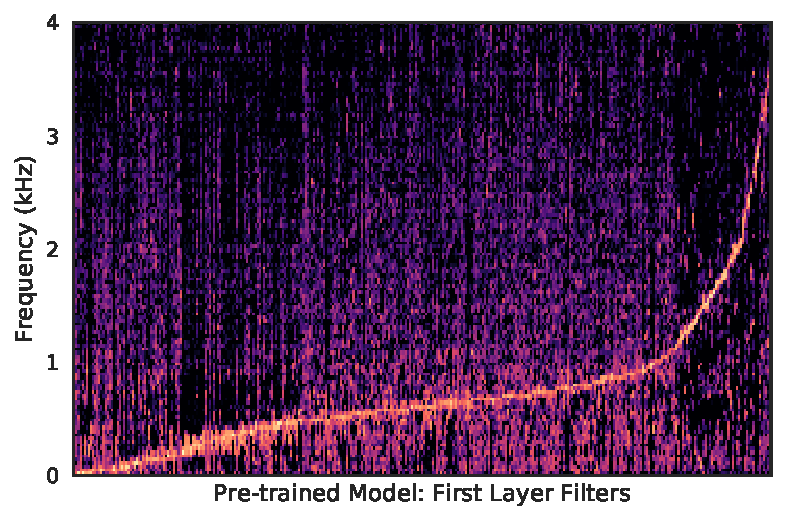
\includegraphics[width=0.6\textwidth]{firstlayer-one.pdf}
	\caption{The first layer filters of the CREPE model trained with six different datasets, visualized using the same method as in Figure \ref{fig:firstlayer}. Compared to the previous cases where the filters are specialized to one dataset, the peak-frequency curve is smoother and covers the full frequency range.}\label{fig:firstlayer-one}
\end{figure}

\subsection{Python Package and Command-Line Interface}

CREPE is distributed as a Python package and is hosted on the Python Package Index (PyPI). It can be installed simply by running the following command:

\vspace{1em}
\texttt{\$ pip install crepe}
\vspace{1em}

\noindent in a Python environment. This command will install the Python package \texttt{crepe} usable in Python scripts as well as a command-line interface that can be called with one or more audio file names:

\vspace{1em}
\texttt{\$ crepe audio\_file.wav}
\vspace{1em}

\noindent The estimated pitch values are saved using the CSV format, like:

\begin{figure}[b]
	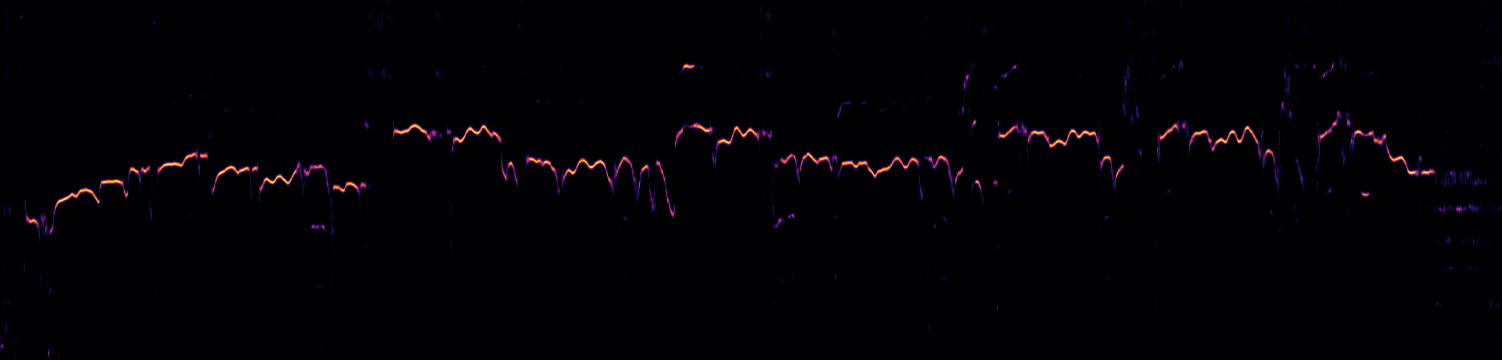
\includegraphics[width=\linewidth]{activation.png}
	\caption{Visualization of the target activation, which can be saved as in image file by using the \texttt{--save-activation} option in the CREPE command-line interface. The audio clip used contains an excerpt of male singing voice.}\label{fig:crepe-activation}
\end{figure}

\vspace{1em}
\texttt{time,frequency,confidence}

\texttt{0.00,185.616,0.907112}

\texttt{0.01,186.764,0.844488}

\texttt{0.02,188.356,0.798015}

\texttt{0.03,190.610,0.746729}

\texttt{0.04,192.952,0.771268}

\texttt{0.05,195.191,0.859440}

\texttt{0.06,196.541,0.864447}

\texttt{0.07,197.809,0.827441}

\texttt{0.08,199.678,0.775208}

\texttt{...}
\vspace{1em}

\noindent where the third column indicates the confidence level of the presence of a pitch, which is obtained by taking the maximum activation value at each frame.

The command-line interface supports various options, such as to use Viterbi smoothing~\cite{viterbi1967decoding} of the pitch curves as in pYIN~\cite{mauch2014pyin} and to save the activation in an image file as shown in Figure \ref{fig:crepe-activation}.
The package contains five pre-trained models with different capacities, where the number of convolutional channels are scaled to 12.5\% (tiny), 25\% (small), 50\% (medium), 75\% (large), or 100\% (full) relative to the model size used in the experiments (see Figure \ref{fig:architecture}), and the specific model capacity to use can be specified using the \texttt{--model-capacity} option.
Smaller-capacity models run significantly faster than the full-capacity model, suitable for resource-constrained use cases where faster computation is preferred at the cost of slightly lower pitch estimation accuracy.


\subsection{Real-Time Web Demo}

In addition to the Python package, we have developed a real-time web demo\footnote{\url{https://marl.github.io/crepe}} where the CREPE model runs on the web browser using the audio recorded from the system microphone and displays the target activation as well as the predicted pitch value in real time.
To enable this, the demo used the W3C Web Audio API for real-time audio input and TensorFlow.js~\cite{smilkov2019tensorflowjs} for running inference on the deep model.
Under the hood, TensorFlow.js uses WebGL which allows GPU acceleration for faster computation of the convolutional layers.
The web demo uses the ``tiny" capacity model in order to run faster in browsers, which uses less than 3\% of the parameters compared to the full model.
The web demo is also open-source and distributed in the same Github repository as the Python package.

\subsection{Argmax-Local Weighted Averaging}

In the process of training the model with diverse datasets, we have observed a side-effect where the model produces more octave errors, i.e. the predicted pitch is an octave apart from the ground truth.
These errors resulted in multiple peaks in the target output vector around the harmonics of the ground-truth frequency, as depicted in Figure \ref{fig:octave-errors}.
When the weighted average over the all 360 bins is used, this ends up predicting a completely different pitch.
To alleviate this, we have revised Equation \ref{eqn:resulting} in the open-source version of CREPE to calculate the weighted average using only the frequency bins around the highest peak in the output:
\begin{equation}\label{eqn:resulting-fixed}
\hat{\cent} = \frac{\sum\limits_{i=m-4}^{m+4}\hat{y}_i \cent_i}{\sum\limits_{i=m-4}^{m+4} \hat{y}_i},
~~~~~~~~~ m = \argmax_i \hat{y}_i.
\end{equation}
Using Equation \ref{eqn:resulting-fixed} improved the transcription accuracies of real-world signals significantly. However, a quantitative evaluation of the robustness in the real-world situations is inherently difficult and is out of the scope of this chapter, because it is virtually impossible to obtain a representative and objective dataset encompassing all such situations.

\begin{figure}
	\centering
	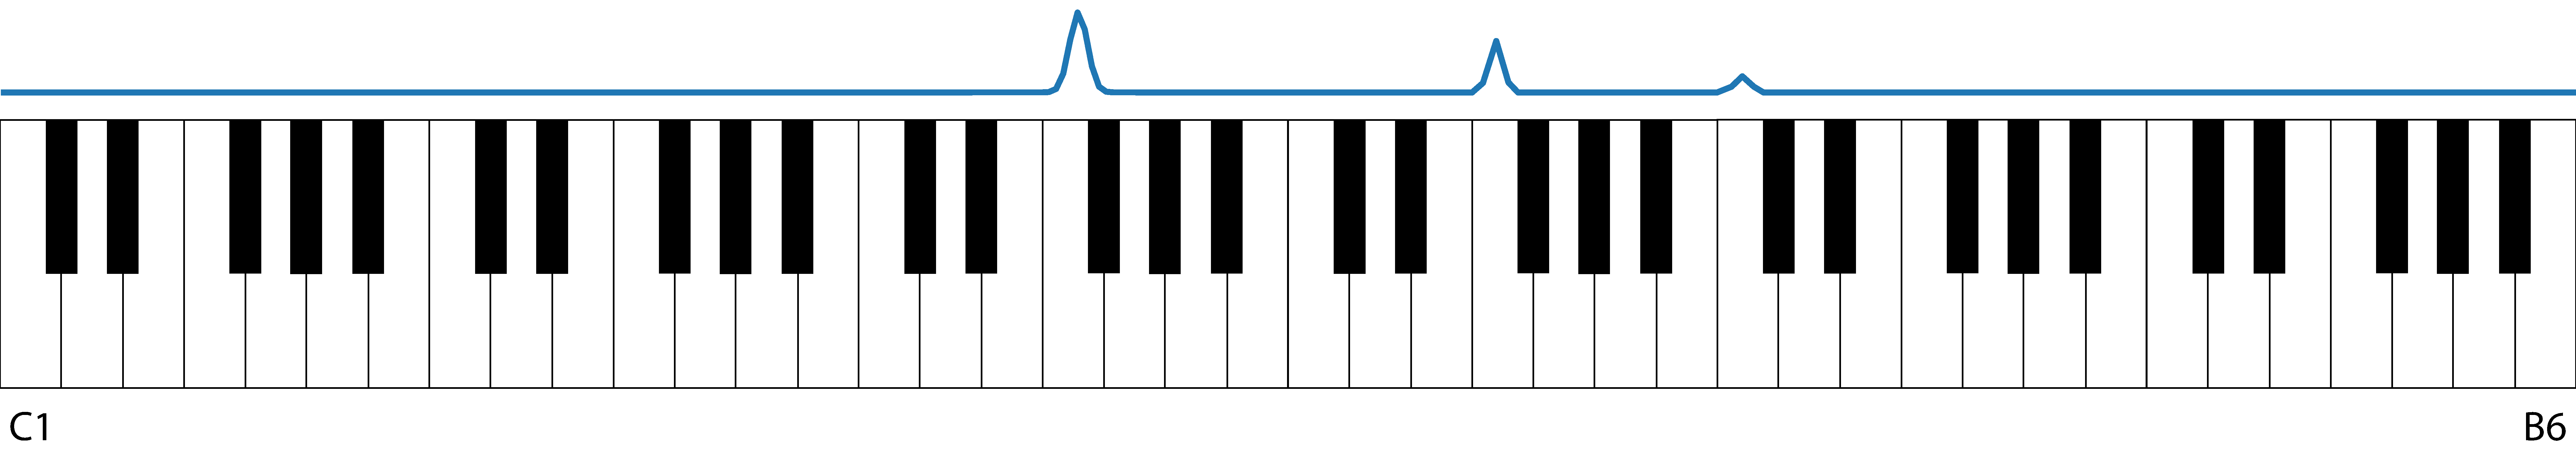
\includegraphics[width=\textwidth]{octave-errors.pdf}
	\caption{An example of an inaccurate target output where there exist multiple peaks around the harmonics of the ground-truth frequency. Equation \ref{eqn:resulting-fixed} ensures that the predicted pitch is calculated using only the frequency bins around the highest peak.}\label{fig:octave-errors}
\end{figure}

\subsection{Data-Driven Models and Real-World Applications}

The series of modifications on the CREPE model are taken in order to release the open-source software that are effective not only for evaluation in an academic setting but also in various real-world scenarios of pitch estimation.
These give an important lesson that should be considered when developing data-driven models for music analysis tasks.
Especially with the rise of deep learning models that typically have a large number of parameters, it is very easy to overfit a model to work well with a specific dataset while not being able to generalize.
This problem can persist even if the dataset is properly splitted for training and evaluation, because it is common for such dataset to have shared characteristics such as recording and mixing conditions that are not particularly representative of the broad range of the real-world data for which the model should supposedly work well.
Therefore, a great amount of care should be taken when selecting the datasets to be used for evaluation of a music analysis model, and qualitative analyses on out-of-distribution real-world data need to be accompanied.


\section{Conclusions}

In this chapter, we presented a novel data-driven method for monophonic pitch tracking based on a deep convolutional neural network operating on time-domain input, CREPE.
We showed that CREPE obtains state-of-the-art results, outperforming pYIN and SWIPE on two datasets with homogeneous and heterogeneous timbre respectively.
Furthermore, we showed that CREPE remains highly accurate even at a very strict evaluation threshold of just 10 cents.
We also showed that in most cases CREPE is more robust to added noise.
In addition, we discussed the challenges that arose during the open-source release of the model, which included how to make the model more generalizable to the real-world sounds and the revised pitch extraction strategy to better deal with increased octave errors.

Ideally, we want the model to be invariant to all transformations that do not affect pitch, such as changes due to distortion and reverberation.
Some invariance can be induced by the architectural design of the model, such as the translation invariance induced by pooling layers in our model as well as in deep image classification models.
However, it is not as straightforward to design the model architecture to specifically ignore other pitch-preserving transformations.
While it is still an intriguing problem to build an architecture to achieve this, we could use data augmentation to generate transformed and degraded inputs that can effectively make the model learn the invariance.
The robustness of the model could also be improved by applying pitch-shifts as data augmentation \cite{mcfee2015muda} to cover a wider pitch range for every instrument.
In addition to data augmentation, various sources of audio timbre can be obtained from software instruments; NSynth \cite{engel2017nsynth} is an example where the training dataset is generated from the sound of software instruments.


Pitch values tend to be continuous over time, but CREPE estimates the pitch of every frame independently without using any temporal tracking, unlike pYIN which exploits this by using an HMM to enforce temporal smoothness.
We can potentially improve the performance of CREPE further by statistically modeling how the pitch value changes over time.
Employing recurrent neural networks (RNNs) is a natural choice for this, and we will explore in the following chapters how RNNs can model the temporal characteristics of music, focusing on two specific tasks: music synthesis (Chapter \ref{ch:synthesis}) and piano transcription (Chapter \ref{ch:adversarial}).


